\titre{27}
\theme{trigo}
\auteur{Nathan Scheinmann}
\niveau{1M}
\source{sesamath-1M-trigo}
\type{serie}
\piments{2}
\pts{}
\annee{2425}

\contenu{
	\tcblower
	\begin{minipage}[t]{0.4\textwidth}{
	\vspace{0pt}
	Un ballon vole à une altitude de $700~\text{m}$ en survolant un lac. Si les angles de dénivellation des rives du lac sont $\alpha=48^\circ$ et $\beta=39^\circ$, trouver la largeur $L$ du lac.
	}
	\end{minipage}
	\hfill
	\begin{minipage}[t]{0.55\textwidth}{
	\vspace{0pt}
	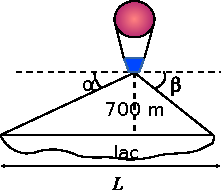
\includegraphics[scale=1]{../medias/1M/trigo/1M-exo-27}
	}
	\end{minipage}
}
\correction{

}

